\documentclass[lecture.tex]{subfiles}

\begin{document}

\exercice{}
%\video{https://youtu.be/blablabla}
\enonce{rdm-0001}{Poutre 3D}

Soit une poutre encastrée sur l’une de ses extrémités en O et libre de l’autre. On négligera l’influence de la pesanteur face aux efforts soumis par la poutre.

\begin{center}
  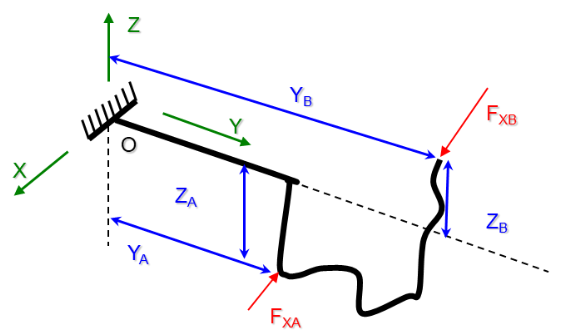
\includegraphics[scale=0.4]{exo-poutre3d.png}
\end{center}

\begin{enumerate}
  \item Faire le bilan des actions mécaniques extérieures à la poutre.
  \item Déterminer le degré d’hyperstatisme de la poutre.
  \item Trouver les inconnus de liaison de la structure (les efforts et les moments résultants de l’encastrement).
  \item Faire l'application numérique pour
  $$\begin{array}{|l|l|}
    \hline
    & \\
    F_{x_A} = 3kN & F_{x_B} = 5kN \\
    & \\
    Y_A = 50cm & Y_B = 90 cm \\
    & \\
    Z_A = 60cm & Z_B = 60 cm \\
    & \\
    \hline
  \end{array}$$
\end{enumerate}

\finenonce{rdm-0001}
\finexercice
\end{document}
